% !TeX program = lualatex
% !TeX root = menu.tex
% !TeX spellcheck = de_DE
\documentclass[a4paper,10pt,notumble]{leaflet}
\usepackage{fontspec}% for lualatex
\usepackage{polyglossia}
\setdefaultlanguage[]{german}
\setotherlanguage[]{german}
%\usepackage[scaled]{helvet}
\renewcommand\familydefault{\sfdefault} 
%\usepackage{setspace}
\usepackage{siunitx}
\sisetup{locale = DE}
\DeclareSIUnit[number-unit-product = { } ]
	\EUR{EUR}

\usepackage{graphicx}

%\usepackage{fontawesome}
% fix the wrong symbols
%\renewcommand{\faHourglass}[1][]{%
%	\faicon{hourglass\if\relax\detokenize{#1}\relax\else-#1\fi}%
%}

\usepackage{titlesec}
\usepackage{hyperref}

\newcommand{\slow}{\faHourglass}

\newcommand{\largemenuonly}[1]{}
\newcommand{\smallmenuonly}[1]{#1}

\newcommand{\meal}[4]{\textbf{#1}\hspace{3mm}%
\begin{minipage}[t]{5.7 cm}
\begin{flushleft}
#2\textsuperscript{ #3}
\end{flushleft}
\end{minipage}%
\hfill\SI{#4}{\EUR}\\[0.3mm]}

\titlespacing*{\section}{0pt}{2mm}{0mm}
%\titlespacing*{<command>}{<left>}{<before-sep>}{<after-sep>}

% Allergen-Verzeichnis
\newcommand{\Getreideprodukte}{a}
\newcommand{\Fisch}{b}
\newcommand{\Krebstiere}{c}
\newcommand{\Schwefel}{d} 
\newcommand{\Sellerie}{e} 
\newcommand{\Laktose}{f} 
\newcommand{\Sesamsamen}{g} 
\newcommand{\Nuss}{h} 
\newcommand{\Eier}{i} 
\newcommand{\Lupinen}{j} 
\newcommand{\Senf}{k} 
\newcommand{\Soja}{l} 
\newcommand{\Weichtiere}{m} 
\newcommand{\Erdnuss}{n} 

\begin{document} 
\hypersetup{
  pdftitle={Speisekarte Yen Yen},  
  pdfsubject={Speisekarte},
  pdfauthor={Jonas Stein}
  pdfnewwindow=true
}

\begin{center}

\includegraphics[width=\textwidth]{gfx/yenyen_head_bw_text.png}
\end{center}

% {\Huge Yen Yen Asia Express}\\
{\small Stand vom \today}\\[4mm]
Unser Restaurant hat an Sonn- und Feiertagen geschlossen. \mbox{Reservierungen} und Vorbestellungen für Selbstabholer unter
\begin{center}
{\Huge 02241 / 126 87 72}\\
\textbf{Wir kochen ohne Glutamat.}
\end{center}

\section*{Partyservice}
Sie möchten Ihre Gäste in Ihrer Location mit gesunden, asiatischen Speisen verwöhnen?\\ 
Sprechen Sie uns an, wir beraten Sie gern.
% !TeX program = lualatex
% !TeX root = menu.tex
% !TeX spellcheck = de_DE
\newpage
\section*{Erste Stärkung}
%\textbf{Vorspeisen}\\
\begin{flushleft}
\meal{X1}{6 Mini-Frühlingsrollen, süßsauer}{\Getreideprodukte,\Soja,\Sellerie}{3.00}
%\meal{X5}{Krabbenchips}{\Getreideprodukte,\Fisch,\Krebstiere}{1.90}
%\meal{X6}{Süßkartoffelchips}{\Getreideprodukte}{2.20}
\meal{X7}{Gebackene Wantan, süßsauer}{\Eier,\Soja,\Getreideprodukte,\Sellerie}{3.70}
\meal{X8}{Gebackener Brokkoli}{\Soja,\Getreideprodukte,\Sellerie,\Eier}{3.70}
%
%\section*{Vorspeisen, auch als Hauptgericht beliebt}
\meal{U1}{Zwei vietnamesische Frühlingsrollen, hausgemacht, süßsauer}{\Getreideprodukte,\Soja,\Eier,\Sellerie}{4.40}
\meal{U2}{Zwei vietnamesische Frühlingsrollen, hausgemacht, pikant}{\Getreideprodukte,\Soja,\Eier,\Sellerie}{4.40}
\meal{U3}{Eine chinesische Frühlingsrolle (groß), hausgemacht, süßsauer}{\Getreideprodukte,\Soja,\Eier,\Sellerie}{4.40}
\meal{U4}{Eine chinesische Frühlingsrolle (groß), hausgemacht, pikant}{\Getreideprodukte,\Soja,\Eier,\Sellerie}{4.40}
\largemenuonly{\newpage}
\vspace{2mm}
%
\section*{Spezialitäten aus Vietnam}
\subsubsection*{Gỏi cuốn} (Vorspeise für 2 Personen)\\
\meal{Y12}{\slow 4 Sommerrollen mit Hühnerfleisch, Garnelen, Ei, Reisnudeln, Hoisin-Erdnuss-Dipp}{\Getreideprodukte,\Eier,\Nuss,\Krebstiere,\Soja}{10.90}
\meal{Y28}{\slow 4 vegane Sommerrollen mit Reisfadennudeln, Möhrchen, Kräuter mit hausgem. Hoisin-Erdnuss-Dipp}{\Getreideprodukte,\Soja}{9.90}
%\largemenuonly{4 Sommerrollen, in hauchdünnes Reispapier eingewickelte, aromatische Kräuter und Salat auf Reisnudeln, 
%	serviert mit einem Hoisin-Erdnuss-Dipp}
\vspace{2mm}
\subsubsection*{Bún Thịt Bò} %Bún Thịt Bò Xào???
\meal{Y27}{\slow {\,} \Phantasiename{Phönixteller} - Reisfadennudeln mit gebr. Rindfleisch, Zwiebeln, Sojasprossen, Kräutern, Limettensoße, Erdnüssen, Gurke \hotpepper}{\Getreideprodukte,\Soja,\Erdnuss,\Krebstiere}{12.90}

\meal{Y2}{\slow\,\Phantasiename{Die vier Jahreszeiten} (Überraschungsgericht)}{\Laktose,\Getreideprodukte,\Soja,\Nuss,\Sesamsamen,\Sellerie}{15.90}
\meal{Y3}{\slow\,\Phantasiename{Drachenteller} - Entenbrustfilet auf gebr. Nudeln mit Gemüse und Cashewkernen \hotpepper}{\Getreideprodukte,\Eier,\Laktose,\Soja,\Nuss}{15.90}

\vspace{2mm}
\subsubsection*{Bún chả giò}
\meal{Y9}{\slow\,\Phantasiename{Zaubertraum} - gebratene Reisfadennudeln mit vietnamesischen Frühlingsrollen, Sojasprossen, Erdnüssen und Limettensoße \hotpepper}{\Getreideprodukte,\Soja,\Eier,\Erdnuss}{14.90}
%
\vspace{2mm}
\subsubsection*{Phở} (vietnamesische Nationalsuppe)
mit Reisbandnudeln, Sojasprossen und Kräutern verfeinert\\
\meal{Y16}{\slow \textellipsis und gedünstetem Rind}{\Getreideprodukte,\Soja}{11.50}
\meal{Y17}{\slow \textellipsis und Huhn}{\Getreideprodukte,\Soja}{10.50}
%
\subsubsection*{Phở xào} Gebratene Reisbandnudeln
mit Gemüse, Kräutern als \textellipsis\\
\meal{Y5}{\slow   \xspace \Phantasiename{Magnolienteller} mit Rind}{\Getreideprodukte,\Soja}{14.90}
\meal{Y6}{\slow   \xspace \Phantasiename{Lilienteller} mit knuspriger Hühnerbrust}{\Getreideprodukte,\Soja}{13.90}
\meal{Y11}{\slow  \xspace \Phantasiename{Amaryllisteller} mit Garnelen \hotpepper}{\Getreideprodukte,\Soja,\Fisch,\Krebstiere}{16.90}
\meal{Y25}{\slow  \xspace \Phantasiename{Orchideenteller} mit kross gebackener Ente}{\Getreideprodukte,\Soja,\Eier}{15.90}
\end{flushleft}
\largemenuonly{\newpage}%
\section*{Suppen}
\meal{Z1}{Pekingsuppe mit Hühnerfleisch}{\Soja,\Getreideprodukte,\Sellerie,\Eier}{3.60}
\meal{Z2}{Wantansuppe}{\Soja,\Getreideprodukte,\Eier}{3,80}
\meal{Z6}{Wantansuppe Thai-Art \hotpepper\hotpepper}{\Getreideprodukte,\Laktose,\Soja,\Eier}{4.90}
\meal{Z8}{Gemüsesuppe}{\Soja}{3,80}
\meal{Z3}{Gemüsesuppe mit Hühnerfleisch}{\Soja}{3,80}
\meal{Z4}{Gemüsesuppe mit Glasnudeln}{\Soja,\Getreideprodukte}{4.10}
\meal{Z7}{Garnelensuppe Thai-Art mit Kokosmilch und Hühnerfleisch \hotpepper\hotpepper (Hauptspeise)}{\Fisch,\Krebstiere,\Getreideprodukte,\Laktose}{14.50}

\vspace{2mm}
\textbf{Hauptgerichte ohne Nudeln werden mit Jasmin-Duftreis serviert}

\section*{Vegetarische Spezialitäten (auf Wunsch auch vegan)}
\meal{V9}{Gebr. Zucchini mit Brokkoli und Knoblauch}{\Getreideprodukte,\Soja}{9.90}
\meal{V10}{Gebr. Blumenkohl mit Zucchini und Frühlingszwiebeln}{\Getreideprodukte,\Soja}{9.90}
\meal{V1}{Tofu mit Gemüse}{\Getreideprodukte,\Soja}{9.90}
\meal{V2}{Tofu mit Gemüse in Curry-Soße}{\Getreideprodukte,\Laktose,\Soja}{10.90}
\meal{V3}{Gebratenes Gemüse}{\Getreideprodukte,\Soja}{7.90}
\meal{V4}{Gebratener Brokkoli mit Zwiebeln und Knoblauch}{\Getreideprodukte,\Soja}{8.90}
\meal{V6}{Gebratener Brokkoli in Currysoße mit Kokosmilch und Blumenkohl}{\Getreideprodukte,\Laktose}{9.90}
\meal{V8}{Gebratenes Gemüse in Curry-Soße}{\Getreideprodukte,\Laktose}{8.90}

\section*{Hühnerfleisch im Teigmantel gebacken}
\meal{H7}{\textellipsis mit Gemüse, süßsauer}{\Eier,\Getreideprodukte,\Soja,\Sellerie}{9.90}
\meal{H8}{\textellipsis mit Gemüse, pikant}{\Eier,\Getreideprodukte,\Soja,\Sellerie}{9.90}

\largemenuonly{\newpage}
\section*{Hühnerfleisch, gebraten}
\meal{H1}{\textellipsis mit gebratenem Reis}{\Getreideprodukte,\Eier,\Soja}{6.90}
\meal{H18}{\textellipsis mit gebr. Reis und Shrimps}{\Getreideprodukte,\Eier,\Soja,\Krebstiere}{9.90}
\meal{H2}{\textellipsis mit gebratenen Nudeln}{\Getreideprodukte,\Eier,\Soja}{6.90}
\meal{H3}{\textellipsis mit Currysoße mit Kokosmilch}{\Laktose,\Getreideprodukte}{9.90}
\meal{H6}{\textellipsis mit Gemüse}{\Getreideprodukte,\Soja}{9.90}
\meal{H9}{\textellipsis mit Gemüse, süßsauer}{\Getreideprodukte,\Sellerie}{9.90}
\meal{H10}{\textellipsis mit Gemüse, herzhaft}{\Getreideprodukte,\Soja,\Sellerie}{9.90}
\meal{H11}{\textellipsis mit Gemüse und Kung Bao-Soße (aus Sojabohnen)}{\Getreideprodukte,\Nuss,\Soja}{9.90}
\meal{H4}{\textellipsis mit Gemüse nach Thai-Art mit Kokosmilch \hotpepper\hotpepper}{\Getreideprodukte,\Soja}{9.90}
\meal{H12}{\textellipsis mit Brokkoli und Knoblauch}{\Getreideprodukte,\Soja}{9.90}
\meal{H13}{\textellipsis mit Ingwer und Zitronengras \hotpepper}{\Getreideprodukte,\Soja}{9.90}
\meal{H15}{\slow \textellipsis als Saté-Spieße mit Erdnuss-Soße und Gemüse \hotpepper}{\Getreideprodukte,\Soja,\Erdnuss,\Laktose}{13.90}


\largemenuonly{\newpage}
\section*{Entenbrustfilet in Teig kross gebraten}
\meal{E1}{\textellipsis mit Gemüse, süßsauer}{\Getreideprodukte,\Sellerie,\Eier,\Soja}{13.90}
\meal{E2}{\textellipsis mit Gemüse, pikant}{\Getreideprodukte,\Sellerie,\Eier,\Soja}{13.90}
\meal{E3}{\textellipsis mit Gemüse und Erdnuss-Soße}{\Getreideprodukte,\Laktose,\Eier,\Erdnuss}{15.90}
\meal{E4}{\textellipsis mit Gemüse und Thaisoße \hotpepper\hotpepper}{\Getreideprodukte,\Laktose,\Eier}{15.90}
\meal{E5}{\textellipsis mit Gemüse und Kung Bao-Soße (aus Sojabohnen) und Cashewkernen}{\Getreideprodukte,\Laktose,\Eier,\Nuss}{15.90}
\meal{E6}{\textellipsis mit Champignons und Zwiebeln, herzhaft}{\Getreideprodukte,\Laktose,\Eier}{15.90}
%\meal{E8}{\textellipsis mit Gemüse, Ingwer und Zitronengras \hotpepper}{\Getreideprodukte,%\Eier}{15.90}
%\meal{E9}
\begin{flushleft}
\largemenuonly{\newpage}

\section*{Spezialitäten vom Rind}
zarte Rinderstreifen kurz angebraten\\
\meal{R1}{\textellipsis mit Gemüse, sehr würzig \hotpepper}{\Getreideprodukte,\Soja,\Sellerie}{12.90}
\meal{R5}{\textellipsis mit Gemüse, mild}{\Getreideprodukte,\Soja}{12.90}
\meal{R3}{\textellipsis mit Gemüse und würziger Soße aus gemahlenen schwarzen Bohnen \hotpepper}{\Getreideprodukte,\Soja,\Laktose}{12.90}
\meal{R4}{\textellipsis mit Zitronengras, Zwiebeln und Ingwer \hotpepper}{\Getreideprodukte,\Soja}{12.90}
\meal{R8}{\textellipsis mit Brokkoli, Zwiebeln, Knoblauch}{\Getreideprodukte,\Soja}{12.90}
\meal{R6}{\textellipsis mit Champignons und Zwiebeln}{\Getreideprodukte,\Soja}{12.90}
\meal{R7}{\textellipsis mit Gemüse nach Thai-Art mit Kokosmilch \hotpepper\hotpepper}{\Getreideprodukte,\Laktose}{14.90}
\meal{R9}{\textellipsis mit Nudeln und Gemüse}{\Getreideprodukte,\Laktose}{14.90}
\largemenuonly{\newpage}

\section*{Spezialitäten aus dem Wasser}
\meal{W9}{\slow Norwegischer Premium-Lachs "mal anders" mit herzhaftem Gemüse}{\Fisch,\Getreideprodukte,\Soja}{16.40}
\meal{W1}{\slow Norwegischer Premium-Lachs mit Gemüse}{\Fisch,\Getreideprodukte,\Soja}{15.40}
%\meal{W2}{\slow \textellipsis und Curry-Soße}{\Fisch,\Getreideprodukte,\Laktose}{15.90}
\meal{W3}{\slow \textellipsis und Kung Bao-Soße (aus Sojabohnen)}{\Fisch,\Getreideprodukte,\Laktose,\Nuss,\Soja}{15.90}
\meal{W11}{\slow Norwegischer Premium-Lachs in hausgemachter Tomatensoße mit Kräutern}{\Fisch,\Getreideprodukte,\Laktose}{16.40}
\meal{W10}{\Phantasiename{Lotusteller} - gebr. Garnelen auf gebr. Reis mit Gemüse und Cashewkernen \hotpepper}{\Getreideprodukte,\Soja,\Krebstiere,\Nuss}{15.90}
\meal{W8}{Garnelen mit Gemüse}{\Getreideprodukte,\Soja,\Krebstiere}{14.50}
\meal{W4}{\textellipsis und Kung Bao-Soße aus Sojabohnen \hotpepper}{\Getreideprodukte,\Soja,\Nuss,\Krebstiere}{14.90}
\meal{W7}{\textellipsis und gebratenen Nudeln}{\Getreideprodukte,\Soja,\Krebstiere}{15.90}
\meal{W5}{Garnelen im Teigmantel gebacken mit Gemüse, süßsauer}{\Eier,\Getreideprodukte,\Soja,\Laktose,\Krebstiere,\Sellerie}{14.50}
\meal{W6}{Garnelen mit Ingwer und Zitronengras \hotpepper}{\Getreideprodukte,\Soja,\Krebstiere}{14.50}

\largemenuonly{\newpage}


\largemenuonly{\newpage}
\section*{Extras als Beilage}
\meal{+K}{Gekochter Reis}{~}{2.00}
\meal{+R}{Gebratener Reis}{~}{2.50}
\meal{+N}{Gebratene Nudeln}{~}{2.50}
\end{flushleft}
\section*{Nachspeisen} 
\meal{N1}{Gebackene Banane mit Honig}{\Getreideprodukte,\Eier}{4.50}
\meal{N4}{Kleines Geheimnis}{\Getreideprodukte,\Eier,\Laktose}{7.50}
%\meal{N5}{Tartufo-Eis mit Schokoladensoße}{\Eier,\Laktose}{3.50}

\largemenuonly{\newpage}
\section*{Kalte Getränke}
\meal{G1}{Cola \SI{0.2}{\litre}}{~}{2.10}
\meal{G3}{Fanta \SI{0.2}{\litre}}{~}{2.10}
\meal{G5}{Wasser \SI{0.2}{\litre}}{~}{2.10}
\meal{G8}{Malzbier \SI{0.33}{\litre})}{~}{2.50}
\meal{G9}{Bitter Lemon \SI{0.2}{\litre})}{~}{2.50}
\meal{G10}{Ginger Ale \SI{0.2}{\litre}}{~}{2.50}
\meal{G11}{Lychee-Nektar \SI{0.2}{\litre}}{~}{2.50}
\meal{G12}{Mango-Nektar \SI{0.2}{\litre}}{~}{2.50}
\meal{G13}{Orangensaft \SI{0.2}{\litre}}{~}{2.50}
\meal{G14}{Apfelsaft \SI{0.2}{\litre}}{~}{2.50}
\section*{Tee und Kaffee}
\meal{J1}{Kaffee}{~}{2.50}
\meal{J11}{Espresso}{~}{2.20}
\meal{J3}{Kamillentee}{~}{2.50}
\meal{J5}{Drachenperlen (Jasmin Tee)}{~}{3.00}
\meal{J12}{Ingwertee frisch geschnitten}{~}{3.50}
\meal{J6}{Schwarzer Tee}{~}{2.50}
\meal{J7}{Blumentee (Kännchen)}{~}{5.90}
\meal{J8}{Grüner Tee}{~}{2.50}
\meal{J9}{Früchtetee}{~}{2.50}
\meal{J10}{Tee aus frischen Minzblättern}{~}{3.50}
\section*{Alkoholische Getränke}
\meal{Q1}{Gaffel Kölsch 4.8\%, \SI{0.33}{\litre}}{~}{2.40}
\meal{Q2}{Bitburger Pils 4.8\%, \SI{0.33}{\litre}}{~}{2.40}
\meal{G7}{Bitburger Pils alkoholfrei, \SI{0.33}{\litre}}{~}{2.40}
\meal{Q3}{Paulaner Weizen 5.5\%, \SI{0.5}{\litre}}{~}{3.60}
\meal{Q8}{Paulaner Weizen alkoholfrei, \SI{0.5}{\litre}}{~}{3.60}
\meal{Q4}{Pflaumenwein 10\%, \SI{0.04}{\litre}}{~}{3.20}
\meal{Q5}{Rotwein Bréjou Bordeaux 12.5\%, \SI{0.2}{\litre}}{~}{4.90}
\meal{Q6}{Weißwein Riesling Kalkstein Qualitätswein Pfalz, tr. 12.5 \%, \SI{0.2}{\litre}}{~}{4.90}
\meal{Q8}{Weißer Burgunder feinherb 11.5 \%, \SI{0.2}{\litre}}{~}{4.90}

\section*{Für Kreative}
Stellen Sie sich Ihr Lieblingsgericht aus den Zutaten der Karte selbst zusammen!
Preis auf Anfrage.
%\newpage
%\vspace{6mm}
\section*{Allergenkennzeichnung}
%\begin{verbatim}
nach EU-Lebensmittelinformationsverordnung: 
\textbf{a} Getreideprodukte (glutenhaltig), 
\textbf{b} Fisch,
\textbf{c} Krebstiere,
\textbf{d} Schwefeldioxide und Sulfite,
\textbf{e} Sellerie,
\textbf{f} Milch und Laktose,
\textbf{g} Sesamsamen,
\textbf{h} Nüsse,
\textbf{i} Eier,
\textbf{j} Lupinen,
\textbf{k} Senf,
\textbf{l} Soja,
\textbf{m} Weichtiere,
\textbf{n} Erdnüsse. 
%\end{verbatim}

Informationen über Zutaten in unseren Speisen, die Allergien
oder Unverträglichkeiten auslösen können, erhalten Sie auf Nachfrage
auch bei unseren Mitarbeitern.\\
\textbf{Gerne passt unser Koch das Rezept auf Ihre Bedürfnisse an.} %
%\vspace{4mm}
%\newpage
\section*{Lage in der Troisdorfer Innenstadt}
\begin{center}
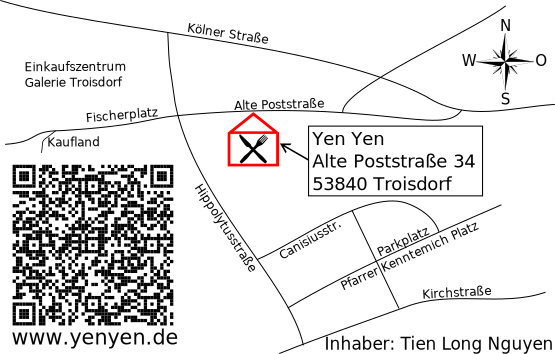
\includegraphics[width=1.0\textwidth]{gfx/map/tdfcity}\\
\end{center}
\end{document}